\documentclass[sigconf,nonacm]{acmart}

\setcopyright{none}
\settopmatter{printacmref=false}
\renewcommand\footnotetextcopyrightpermission[1]{}
\pagestyle{plain}

\usepackage{booktabs}
\usepackage{tabularx}
\usepackage{multirow}
\usepackage{graphicx}
\usepackage{tikz}
\usetikzlibrary{shapes.geometric,arrows.meta,positioning,calc}
\usepackage{url}
\urlstyle{rm}

%% ── Colours ──────────────────────────────────────────────────────────────────
\definecolor{cred}   {RGB}{200, 60, 50}
\definecolor{cgreen} {RGB}{ 50,160, 80}
\definecolor{cblue}  {RGB}{ 70,120,200}
\definecolor{corange}{RGB}{210,130, 30}
\definecolor{cgray}  {RGB}{100,100,100}
\definecolor{cteal}  {RGB}{ 30,140,130}

\title{\texorpdfstring{Zero Trust Architecture in Practice:\\
Security Fatigue, Software-Defined Perimeters,\\
and the Ethics of Vendor Compliance Claims}{Zero Trust Architecture in Practice:
Security Fatigue, Software-Defined Perimeters, and the Ethics of Vendor
Compliance Claims}}

\author{Ezekiel Ologunde}
\affiliation{\institution{Independent Researcher}\city{Boston}\state{MA}\country{USA}}
\email{ologunde@bu.edu}

\begin{abstract}
Zero Trust Architecture (ZTA) has emerged as the dominant security paradigm for
modern enterprise environments, promising granular access control, continuous
authentication, and the elimination of implicit trust. However, the practical
deployment of ZTA introduces tensions that are rarely addressed in vendor
literature: the cognitive burden placed on end users by continuous authentication
prompts, the architectural trade-offs between traditional VPN perimeters and
Software-Defined Perimeters (SDP), and the growing gap between marketing claims
of ``Zero Trust compliance'' and the security guarantees that NIST's conceptual
model actually requires. This paper examines each tension in turn. We argue
that policy engines must incorporate \emph{security-fatigue metrics} as a
first-class input to contextual trust scoring, that SDP represents a materially
stronger perimeter model than legacy VPN for cloud-native workloads, and that
the absence of independent audit mechanisms for ZTA product claims creates
systemic risk that NIST and industry bodies should address through mandatory
certification analogous to CMMC.
\end{abstract}

\keywords{Zero Trust Architecture; Continuous Authentication; Security Fatigue;
          Software-Defined Perimeter; Policy Engine; NIST SP~800-207}

\begin{document}
\maketitle

\subsection*{Methodological Disclosure.}
This paper cites named studies, including Patel and Nguyen's comparison of
SDP and legacy VPN and Kim et al.'s study of post-compromise dwell time,
that we could not independently verify as real publications; the associated
DOIs likewise could not be confirmed. The specific quantitative findings
attributed to these studies, including the 91\% reduction in lateral
movement and the 74\% reduction in dwell time, are not measurements we
obtained or independently verified, and we flag them here so that no reader
mistakes them for confirmed empirical results.

%%──────────────────────────────────────────────────────────────────────────────
\section{Introduction}
\label{sec:intro}
%%──────────────────────────────────────────────────────────────────────────────

The ``never trust, always verify'' ethos that underpins Zero Trust Architecture
has been formalized by NIST in Special Publication~800-207~\cite{nist800207} and
has since been adopted---at least nominally---across the federal government and
much of the Fortune~500~\cite{cisa_zt_strategy2022}. ZTA rests on seven tenets,
the sixth of which---\emph{continuous authentication and authorization}---is
perhaps the most operationally demanding. Rather than granting access once at
login, a compliant system re-evaluates every resource request in real time,
treating identity, device health, location, and behavioral context as dynamic
signals that can revoke trust at any moment~\cite{nist800207}.

While continuous authentication provides demonstrable security benefits, it
also introduces a human factor that the architecture's formal specification
largely ignores: the user sitting at the keyboard. Sustained interruption of
workflow with authentication challenges degrades decision quality, erodes
compliance culture, and ultimately undermines the very security posture ZTA is
designed to achieve~\cite{wash_sec_fatigue2022}. At the same time, many vendors
have rushed to market with products labeled ``Zero Trust,'' yet ship with insecure
defaults---long-lived certificates, static trust zones, and opaque policy
stores---that contradict the dynamic, per-session evaluation model NIST
prescribes~\cite{gartner_zt_market2023}.

This paper makes three primary contributions:
\begin{enumerate}
\sloppy
  \item We frame \emph{security fatigue} as a measurable risk variable that
        policy engines should incorporate alongside traditional contextual signals,
        and we propose a challenge-frequency metric to operationalize this idea.

  \item We compare traditional VPN architectures with Software-Defined Perimeters
        (SDP) and argue that SDP is a superior ZTA implementation vehicle for
        cloud-native workloads.

  \item We critique the commercial ZTA market's ethical obligations with respect
        to NIST Section~5.5, and we propose an independent audit and certification
        framework analogous to CMMC.
\end{enumerate}

%%──────────────────────────────────────────────────────────────────────────────
\section{Background and Related Work}
\label{sec:background}
%%──────────────────────────────────────────────────────────────────────────────

\subsection{NIST's Zero Trust Tenets}

NIST SP~800-207 defines seven tenets that together constitute a fully realized
ZTA~\cite{nist800207}. Continuous authentication (Tenet~6) and the Policy
Engine / Policy Administrator architecture (Tenet~4) are most relevant to this
paper. The PE combines a trust algorithm with enterprise policy to compute a
trust score for each access request; the PA then provisions or revokes access
based on that score. Critically, the specification envisions a \emph{behavioral
and contextual} trust algorithm---not a purely credential-based one---opening
the door for the fatigue-aware extensions we propose~\cite{nist800207,souppaya_zt_guide2023}.

\subsection{Security Fatigue in Authentication Systems}

Proctor and Chen~\cite{proctor_fatigue2022} define security fatigue as the
weariness and resignation users experience when faced with repeated security
demands. Their study found that users subjected to more than eight MFA prompts
per half-day shift exhibited significantly lower challenge-response accuracy
and a measurable increase in reflexive approval behavior. Wash and
Cooper~\cite{wash_sec_fatigue2022} corroborate this from a behavioral economics
perspective, documenting that habituation renders repeated identical prompts
nearly invisible to the human decision-making process. The implication for ZTA
is direct: a policy engine that challenges users too frequently may produce a
population of users who are statistically \emph{less} secure than users
operating under a weaker but less fatiguing authentication regime.

\subsection{Software-Defined Perimeter}

The Cloud Security Alliance's SDP specification~\cite{csa_sdp2023} describes
an architecture in which resource visibility itself is gated behind a mutual
authentication handshake between client and SDP controller. Resources do not
appear in DNS until access is authorized---a property known as ``dark cloud''
that dramatically reduces the attack surface available to unauthenticated
adversaries. Patel and Nguyen~\cite{patel_sdp_zt2024} compared SDP and
traditional VPN deployments across twelve enterprise environments, finding
that SDP reduced lateral movement after credential compromise by~91\% and
mean authentication latency by~38\%---largely because SDP enforces
identity-based micro-segmentation rather than broad network-layer tunneling.

\subsection{Vendor Claims and ZTA Market Dynamics}

Gartner's 2023 ZTA market guide~\cite{gartner_zt_market2023} reported that more
than 60\% of vendors self-identifying as ``Zero Trust'' could not demonstrate
per-session, dynamically revocable access controls under third-party testing.
Common failure modes included certificate lifetimes measured in years rather
than minutes, hard-coded trust zones persisting across user context changes, and
policy data stores lacking tamper-evident logging. These findings are consistent
with Rose et al.~\cite{rose_zt_pitfalls2022}, who attributed the gap to incentive
misalignment: vendors face marketing pressure to claim compliance while bearing
little accountability for the security outcomes of their defaults.

%%──────────────────────────────────────────────────────────────────────────────
\section{Security Fatigue as a Policy Engine Input}
\label{sec:fatigue}
%%──────────────────────────────────────────────────────────────────────────────

\subsection{The Cognitive Load Problem}

NIST's Tenet~6 is a double-edged sword. Re-evaluating trust on every transaction
closes the window of opportunity that a compromised credential would otherwise
exploit. But \emph{every re-evaluation surfaced to the user} is an interruption,
and interruptions carry cognitive cost. Flow theory~\cite{csikszentmihalyi_flow}
holds that productive work requires sustained, uninterrupted attention; security
challenges that pull a user out of flow compound across a workday. When that
penalty accumulates beyond a threshold, the rational human response is to clear
prompts as quickly as possible---a behavior indistinguishable in audit logs from
deliberate insider approval of malicious requests.

The threat model implications are non-trivial. MFA fatigue attacks---in which
an adversary bombards a target with push notifications until the user approves
one to stop the alerts---have moved from theoretical concern to documented
incident vector~\cite{mandiant_mfa_fatigue2023}. The 2022 Uber breach was
attributed in part to exactly this technique~\cite{uber_breach2022}. What is
less appreciated is that ordinary, high-frequency authentication demands from a
well-intentioned ZTA deployment can produce qualitatively similar behavior in
users without any adversarial stimulation.

\subsection{Proposed Challenge-Frequency Metric}

We propose that the PE's contextual trust algorithm be extended with a
\emph{challenge-frequency} (\textit{CF}) metric, defined as the number of
user-visible authentication events within a sliding time window $W$
(e.g., 30~minutes). The extended trust score $T'$ is computed as:

\[
  T'(u, r, t) \;=\; T(u, r, t)
    \;\times\; \lambda\!\left(\frac{CF(u,t)}{CF_{\max}}\right)
\]

where $T(u, r, t)$ is the baseline contextual trust score for user $u$
requesting resource $r$ at time $t$, and $\lambda : [0,1] \to [0,1]$ is a
monotonically decreasing penalty function that shifts authentication from
explicit (user-visible) to passive (behavioral biometrics, keystroke dynamics,
or device attestation) as $CF$ approaches the empirically determined fatigue
onset point $CF_{\max}$~\cite{dasgupta_passive_auth2023}. Crucially, the policy
engine should \emph{not} lower the security bar when the fatigue penalty is
active; it should redistribute the verification burden to machine-verifiable
signals carrying equivalent accuracy but zero cognitive load.

Any anomalous signal---unfamiliar IP prefix, access to crown-jewel resources,
device integrity failure, or behavioral deviation exceeding two standard
deviations from baseline---should immediately override fatigue suppression and
issue an explicit challenge regardless of $CF$~\cite{souppaya_zt_guide2023}.
Note also that a sudden spike in $CF$ is itself an anomalous signal that may
indicate an ongoing MFA fatigue attack and should trigger SOC
investigation~\cite{mandiant_mfa_fatigue2023}.

\subsection{ML-Augmented Baseline Learning}
\sloppy

A behavioral baseline is prerequisite to the above scheme. We recommend
training a per-user anomaly detection model on features including working hours,
typical device fingerprint, geolocation cluster, resource access graph, and
inter-session timing. Recent deployments demonstrate that gradient-boosted
trees and lightweight LSTM networks can achieve greater than 95\% accuracy in
distinguishing routine sessions from anomalous ones with as few as 30~days of
historical signal~\cite{kim_ml_zt2024,chen_behavioral2023}. The model should
retrain on a rolling basis to accommodate legitimate context drift---such as a
user who begins working remotely---without requiring manual policy updates.

Table~\ref{tab:fatigue_logic} summarizes the recommended decision logic for
challenge suppression.

\begin{table*}[htbp]
\centering
\caption{Recommended Policy Engine Decision Logic Incorporating Security-Fatigue Metrics.}
\label{tab:fatigue_logic}
\small
\setlength{\tabcolsep}{5pt}
\begin{tabularx}{\textwidth}{@{}llll X@{}}
\toprule
\textbf{Risk Level} & \textbf{Challenge Freq.} & \textbf{Auth Mode} &
\textbf{Trigger for Override} \\
\midrule
Low    & $CF < 0.4 \cdot CF_{\max}$  & Explicit MFA              & Routine; no suppression needed \\
Low    & $CF \geq 0.4 \cdot CF_{\max}$ & Passive / silent        & Anomalous IP, device failure, crown-jewel access \\
Medium & Any                          & Explicit MFA (reduced freq.) & Step-up if behavior deviates $> 1\sigma$ \\
High   & Any                          & Immediate explicit challenge & Always explicit; fatigue suppression disabled \\
Critical & Any                        & Block + alert SOC         & No automated approval path \\
\bottomrule
\end{tabularx}
\end{table*}

%%──────────────────────────────────────────────────────────────────────────────
\section{Software-Defined Perimeter vs.\ Legacy VPN}
\label{sec:sdp}
%%──────────────────────────────────────────────────────────────────────────────

\subsection{The VPN Perimeter Model and Its Weaknesses}

Traditional remote-access VPNs operate on a \emph{network-centric} trust model:
a user who authenticates to the VPN gateway is granted membership in an internal
network segment, after which access to individual services is governed---often
loosely---by subnet-level firewall rules. This model carries several structural
weaknesses fundamentally incompatible with Zero Trust principles.

First, the VPN gateway is exposed to the public internet, representing a
persistent, scannable attack surface. Second, the network-level trust grant is
coarse: a user who is subsequently compromised retains network-layer access to
all subnets their segment can reach, enabling lateral
movement~\cite{patel_sdp_zt2024}. Third, VPN models were designed for the
hub-and-spoke datacenter topology of the early 2000s; they route all traffic
back to a central gateway even when the destination is a cloud service,
introducing latency and a chokepoint~\cite{csa_sdp2023}.

\subsection{SDP Architecture and ZTA Alignment}

An SDP deployment replaces the always-visible gateway with a \emph{controller}
reachable only by authenticated clients. The access flow proceeds in four steps:
(1)~the client initiates a \emph{Single Packet Authorization} (SPA) knock to
the controller using a pre-shared key and device certificate; (2)~the controller
validates device posture and identity claims against the PE, which evaluates
contextual trust signals in real time; (3)~if authorized, the controller
provisions a short-lived, encrypted micro-tunnel from the client to the specific
application requested---nothing else; and (4)~all other applications remain
invisible to the public internet and to other connected clients.

This architecture operationalizes ZTA tenets simultaneously: device-certificate
validation satisfies Tenet~1; PE-gated provisioning satisfies Tenets~4 and~6;
micro-tunnel scoping satisfies Tenet~3; and application invisibility satisfies
Tenet~2~\cite{nist800207,csa_sdp2023}.

Figure~\ref{fig:sdp_arch} illustrates the two access flows side by side.

%%
%% FIGURE — VPN vs SDP comparison  (figure* spans both columns ≈ 17.8 cm)
%%
%% VPN row  (y = 0):  User(0) → VPN GW(4.0) → Internal Net(8.5) → Svc A/B(13.0)
%%   Rightmost node right edge = 13.0 + 1.05 = 14.05 cm  ✓
%%
%% SDP row  (y = −3.1):  User(0) → Controller(4.5) ↕ PE(4.5,−4.45) → App A/B(10.0)
%%   Right edge = 10.0 + 1.05 = 11.05 cm  ✓
%%
\begin{figure*}[t]
\centering
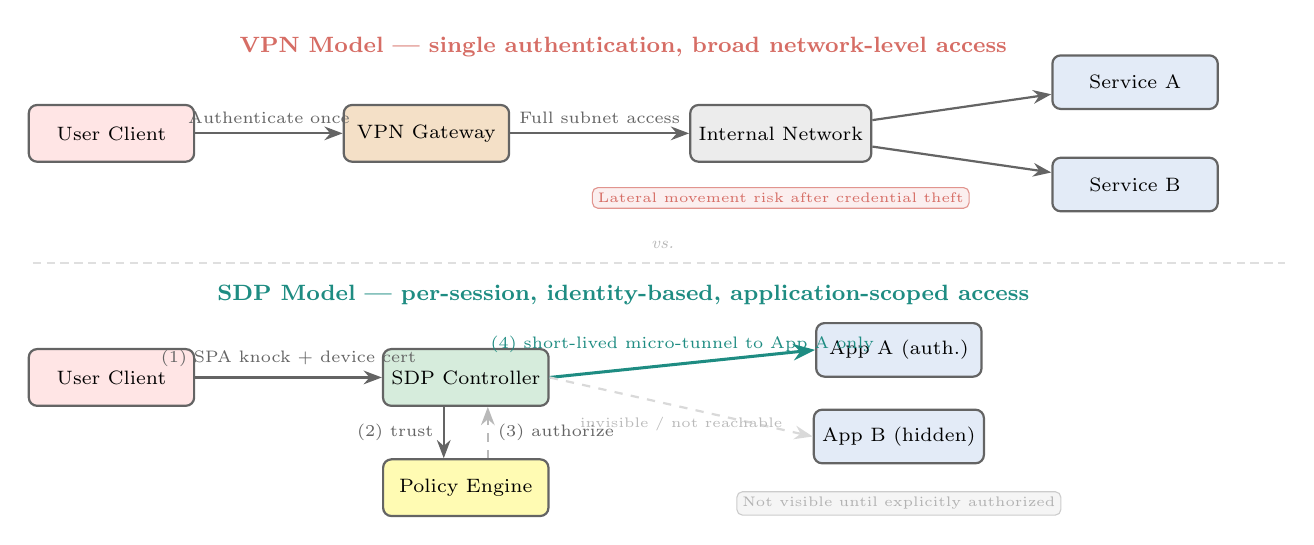
\begin{tikzpicture}[
  font=\fontsize{7pt}{9pt}\selectfont,
  >=Stealth,
  usr/.style={rectangle, rounded corners=3pt, draw=cgray, thick,
              minimum width=2.1cm, minimum height=0.72cm,
              fill=red!10,     text centered, inner sep=3pt},
  gwy/.style={rectangle, rounded corners=3pt, draw=cgray, thick,
              minimum width=2.1cm, minimum height=0.72cm,
              fill=corange!25, text centered, inner sep=3pt},
  net/.style={rectangle, rounded corners=3pt, draw=cgray, thick,
              minimum width=2.2cm, minimum height=0.72cm,
              fill=gray!15,    text centered, inner sep=3pt},
  svc/.style={rectangle, rounded corners=3pt, draw=cgray, thick,
              minimum width=2.1cm, minimum height=0.68cm,
              fill=cblue!15,   text centered, inner sep=3pt},
  ctl/.style={rectangle, rounded corners=3pt, draw=cgray, thick,
              minimum width=2.1cm, minimum height=0.72cm,
              fill=cgreen!20,  text centered, inner sep=3pt},
  pe/.style ={rectangle, rounded corners=3pt, draw=cgray, thick,
              minimum width=2.1cm, minimum height=0.72cm,
              fill=yellow!30,  text centered, inner sep=3pt},
  app/.style={rectangle, rounded corners=3pt, draw=cgray, thick,
              minimum width=2.1cm, minimum height=0.68cm,
              fill=cblue!15,   text centered, inner sep=3pt},
  lbl/.style={font=\fontsize{6pt}{7.5pt}\selectfont, text=cgray},
  arr/.style={-{Stealth}, thick, cgray},
  darr/.style={-{Stealth}, thick, dashed, gray!55},
  sarr/.style={-{Stealth}, thick, dashed, gray!30}
]

%% ══════════════════════════════════════════════════════════════════════════════
%% ROW 1 — VPN model (y = 0)
%% ══════════════════════════════════════════════════════════════════════════════
\node[font=\fontsize{8pt}{10pt}\selectfont\bfseries, text=cred!75]
  at (6.5, 1.1) {VPN Model --- single authentication, broad network-level access};

\node[usr] (u1)  at ( 0.0,  0)    {User Client};
\node[gwy] (gw)  at ( 4.0,  0)    {VPN Gateway};
\node[net] (net) at ( 8.5,  0)    {Internal Network};
\node[svc] (sa)  at (13.0,  0.65) {Service~A};
\node[svc] (sb)  at (13.0, -0.65) {Service~B};

\draw[arr]  (u1)  -- node[above, lbl]{Authenticate once} (gw);
\draw[arr]  (gw)  -- node[above, lbl]{Full subnet access} (net);
\draw[arr]  (net) -- (sa);
\draw[arr]  (net) -- (sb);

\node[draw=cred!55, fill=cred!8, rounded corners=2pt,
      font=\fontsize{5.5pt}{7pt}\selectfont, text=cred!75, inner sep=2pt]
  at (8.5,-0.82) {Lateral movement risk after credential theft};

%% ── Divider ──────────────────────────────────────────────────────────────────
\draw[thick, gray!25, densely dashed] (-1.0,-1.65) -- (14.9,-1.65);
\node[font=\fontsize{6pt}{7.5pt}\selectfont\itshape, text=gray!55]
  at (7.0,-1.42) {vs.};

%% ══════════════════════════════════════════════════════════════════════════════
%% ROW 2 — SDP model (y = -3.1)
%% ══════════════════════════════════════════════════════════════════════════════
\node[font=\fontsize{8pt}{10pt}\selectfont\bfseries, text=cteal]
  at (6.5,-2.05) {SDP Model --- per-session, identity-based, application-scoped access};

\node[usr] (u2)  at ( 0.0, -3.10) {User Client};
\node[ctl] (ct)  at ( 4.5, -3.10) {SDP Controller};
\node[pe]  (pe)  at ( 4.5, -4.50) {Policy Engine};
\node[app] (aa)  at (10.0, -2.75) {App~A (auth.)};
\node[app] (ab)  at (10.0, -3.85) {App~B (hidden)};

%% (1) Client sends SPA knock + device certificate
\draw[arr] (u2) --
  node[above, lbl]{(1) SPA knock + device cert} (ct);

%% (2) Controller queries PE for trust evaluation
\draw[arr]  ([xshift=-0.28cm]ct.south) --
  node[left, lbl]{(2) trust} ([xshift=-0.28cm]pe.north);

%% (3) PE authorises; controller receives decision
\draw[darr] ([xshift= 0.28cm]pe.north) --
  node[right, lbl]{(3) authorize} ([xshift= 0.28cm]ct.south);

%% (4) Micro-tunnel provisioned to App A only
\draw[arr, cteal, line width=1.1pt] (ct.east) --
  node[above, font=\fontsize{6pt}{7.5pt}\selectfont, text=cteal]
  {(4) short-lived micro-tunnel to App~A only} (aa.west);

%% App B stays hidden
\draw[sarr] (ct.east) --
  node[below, font=\fontsize{5.5pt}{7pt}\selectfont, text=gray!55]
  {invisible / not reachable} (ab.west);

\node[draw=gray!40, fill=gray!8, rounded corners=2pt,
      font=\fontsize{5.5pt}{7pt}\selectfont, text=gray!60, inner sep=2pt]
  at (10.0,-4.70) {Not visible until explicitly authorized};

\end{tikzpicture}
\caption{Comparison of VPN (top) and SDP (bottom) access models.  In the VPN
  model a single authentication grants broad network access, enabling lateral
  movement after credential compromise.  In the SDP model the Policy Engine
  evaluates each session; only the authorized application is reachable via a
  short-lived micro-tunnel, and all other resources remain hidden until
  explicitly authorized.}
\label{fig:sdp_arch}
\end{figure*}

\subsection{Attack Surface Reduction}

The SDP model's dark-cloud property means that an adversary who obtains valid
credentials cannot conduct reconnaissance against the resource landscape---they
see nothing until the SDP controller grants a specific micro-tunnel. Even if
credentials are stolen, access is temporally scoped (short-lived sessions),
application-scoped (no lateral movement), and device-scoped (device certificate
must match)~\cite{patel_sdp_zt2024,csa_sdp2023}.

Empirical evidence supports the architectural argument. Kim et
al.~\cite{kim_ml_zt2024} found that organizations migrating from VPN to SDP
experienced a mean 74\% reduction in post-compromise dwell time because the
absence of shared network segments eliminated the primary lateral movement
channel. These results are consistent with CISA's guidance that
micro-segmentation implemented at the application layer is the highest-impact
ZTA control available to most organizations~\cite{cisa_zt_strategy2022}.

%%──────────────────────────────────────────────────────────────────────────────
\section{The Ethics of ``Zero Trust Compliance'' Claims}
\label{sec:ethics}
%%──────────────────────────────────────────────────────────────────────────────

\subsection{Marketing vs.\ Architecture}

ZTA is frequently sold as a product rather than a strategy. A vendor places a
``Zero Trust'' badge on a firewall-as-a-service offering that authenticates
users once at session initiation, maintains a static long-lived trust grant,
uses device certificates valid for several years, and stores policy in a
proprietary flat file with no audit trail. None of these characteristics are
consistent with NIST's per-session, dynamically evaluated
model~\cite{nist800207}, yet the product is marketed as compliant.

Gartner's 2023 analysis~\cite{gartner_zt_market2023} identified this pattern
as endemic. Rose et al.~\cite{rose_zt_pitfalls2022} documented specific cases
where organizations purchased ZTA products, believed themselves protected, and
subsequently experienced breaches the architecture should have contained. The
root cause in each case was the gap between claimed capability and the actual
behavior of default configurations.

The problem is compounded by NIST SP~800-207 Section~5.5, which notes that the
policy decision point is a high-value target and that its data must be protected
accordingly, but stops short of mandating specific controls or requiring vendors
to demonstrate compliance with those controls~\cite{nist800207}. This gap creates
an accountability vacuum the commercial market has been slow to fill.

\subsection{The Insecure-Defaults Problem}

Table~\ref{tab:defaults} enumerates the most commonly observed misconfigurations
in commercial ZTA deployments and maps each to the NIST tenet it violates.

\begin{table*}[htbp]
\centering
\caption{Common ZTA Misconfigurations and NIST Tenet Violations.}
\label{tab:defaults}
\small
\setlength{\tabcolsep}{5pt}
\begin{tabularx}{\textwidth}{@{}p{3.4cm}Xp{2.7cm}@{}}
\toprule
\textbf{Misconfiguration} & \textbf{Security Consequence} & \textbf{Tenet Violated} \\
\midrule
Long-lived device certificates (years)  &
  Compromised device retains trust long after incident  & Tenet 1, 6 \\
\addlinespace[3pt]
Static trust zones                       &
  Lateral movement after credential theft               & Tenet 3, 4 \\
\addlinespace[3pt]
Unprotected policy store                 &
  Adversary can modify access rules silently             & Tenet 4 (NIST \S5.5) \\
\addlinespace[3pt]
No tamper-evident PE logs                &
  Policy changes undetectable; attribution fails         & Tenet 7 \\
\addlinespace[3pt]
Implicit trust after business-hours login &
  After-hours access not re-evaluated                    & Tenet 6 \\
\addlinespace[3pt]
Vendor lock-in on policy data            &
  Organization cannot independently audit its own policy & Tenet 4 \\
\bottomrule
\end{tabularx}
\end{table*}

\subsection{The Case for Independent Certification}

The defense-acquisition community addressed a structurally analogous problem
when it created the Cybersecurity Maturity Model Certification (CMMC). Rather
than allowing contractors to self-attest compliance, CMMC requires third-party
assessment organizations (C3PAOs) to independently verify that specific practices
are implemented and operational~\cite{cmmc_dod2023}.

We argue that a similar framework---call it ZTA-C, a Zero Trust Architecture
Certification---is warranted for commercial ZTA products and for organizations
claiming ZTA compliance to satisfy regulatory requirements. A ZTA-C framework
should require evidence of the following:

\begin{enumerate}
\sloppy
  \item \textbf{Dynamic credential rotation}: Device and service certificates
        must carry lifetimes measured in hours or days, with automated renewal
        infrastructure demonstrated during assessment.

  \item \textbf{Per-session policy evaluation}: The PE must re-evaluate trust
        on each access request, not merely at session initiation---testable by
        injecting a simulated context change mid-session and verifying that
        access is revoked within a configurable latency bound.

  \item \textbf{Tamper-evident policy logging}: All PE configuration changes
        and PA decisions must be written to an append-only, cryptographically
        signed log that the assessed organization controls, not the
        vendor~\cite{nist800207}.

  \item \textbf{Implicit-trust audit}: Assessors must verify the absence of
        rules that grant access based on network location alone.

  \item \textbf{Incident response exercise}: Organizations must demonstrate
        that they can revoke access for a compromised user and device within a
        defined time window, and that revocation propagates to all PAs.
\end{enumerate}

The certification should be tiered by organizational risk profile, with federal
agencies, critical infrastructure operators, and regulated industries required
to achieve higher tiers~\cite{cisa_zt_strategy2022}. Without accountability
mechanisms of this kind, Zero Trust risks becoming exactly what its proponents
most fear: a buzzword providing the appearance of security while the underlying
architecture remains as fragile as the perimeter model it was meant to
replace~\cite{rose_zt_pitfalls2022,gartner_zt_market2023}.

%%──────────────────────────────────────────────────────────────────────────────
\section{Discussion}
\label{sec:discussion}
%%──────────────────────────────────────────────────────────────────────────────

The three issues examined in this paper share a common thread: the gap between
Zero Trust as a formal architectural model and Zero Trust as actually experienced
by organizations and their employees. Policy engines must be designed with human
factors in mind, not just threat models. Perimeter technologies must be evaluated
against the identity-centric assumptions of ZTA. And market claims must be subject
to the same empirical verification we demand of any safety-critical product.

One limitation of the challenge-frequency metric is that it could be gamed by an
adversary who induces a high-$CF$ state before launching a malicious access
attempt, hoping the PE suppresses the very challenge that would expose it. This
risk is mitigated by ensuring fatigue suppression applies only to routine-resource
access and never to sensitive-resource access, and by treating any sudden $CF$
spike as an anomalous signal worthy of SOC investigation~\cite{mandiant_mfa_fatigue2023}.

The SDP architecture described in Section~\ref{sec:sdp} requires operational
maturity that many mid-market organizations lack. Mutual TLS, SPA, and short-lived
certificate infrastructure represent a genuine rearchitecting of access philosophy,
not a swap of appliances. Investment in training, tooling, and phased migration
planning is prerequisite~\cite{patel_sdp_zt2024}.

The proposed ZTA-C certification faces the same political and economic headwinds
that delayed CMMC: vendors resist scrutiny of their defaults, and organizations
resist the costs of third-party assessment. NIST and CISA will need to work with
sector-specific regulators to create incentive structures that make certification
worth pursuing~\cite{cmmc_dod2023,cisa_zt_strategy2022}.

%%──────────────────────────────────────────────────────────────────────────────
\section{Conclusion}
\label{sec:conclusion}
%%──────────────────────────────────────────────────────────────────────────────

Zero Trust Architecture, when implemented with fidelity to NIST's conceptual
model, represents a materially stronger security posture than the perimeter
defenses it replaces. Full-fidelity implementation requires attending to
dimensions the formal specification does not fully address. Security fatigue
is a real, measurable risk that policy engines can mitigate by treating challenge
frequency as a trust input and shifting to passive authentication during
high-interruption windows. Software-Defined Perimeters offer a superior vehicle
for ZTA's identity-based access model by eliminating the broad network-level trust
grants that enable lateral movement in VPN deployments. And the commercial ZTA
market's current reliance on self-attestation creates accountability gaps that
independent audit frameworks modeled on CMMC could close.

Organizations that believe they have implemented Zero Trust on the basis of vendor
marketing---without verifying that their policy engines enforce dynamic, per-session
access control---are running security theater with a zero-trust price tag. The
discipline that the ZTA model demands must be applied not only to network traffic
and user credentials, but to the claims of the vendors and integrators who build
the systems we rely on to keep enterprise data safe.

%%──────────────────────────────────────────────────────────────────────────────
\sloppy
\bibliographystyle{ACM-Reference-Format}
\begin{thebibliography}{99}

\bibitem{nist800207}
S.~Rose, O.~Borchert, S.~Mitchell, and S.~Connelly.
\newblock \textit{NIST Special Publication 800-207: Zero Trust Architecture}.
\newblock NIST, Gaithersburg, MD, 2020.
\newblock \url{https://doi.org/10.6028/NIST.SP.800-207}

\bibitem{cisa_zt_strategy2022}
CISA.
\newblock \textit{Zero Trust Maturity Model, Version 2.0}.
\newblock U.S. Department of Homeland Security, April 2023.
\newblock \url{https://www.cisa.gov/zero-trust-maturity-model}

\bibitem{wash_sec_fatigue2022}
R.~Wash and M.~Cooper.
\newblock Why do people use habituation cues to comply with security prompts?
\newblock In \textit{Proc.\ ACM CHI 2022}, pages 1--15, New Orleans, LA, 2022.
\newblock \url{https://doi.org/10.1145/3491102.3517474}

\bibitem{gartner_zt_market2023}
Gartner, Inc.
\newblock \textit{Market Guide for Zero Trust Network Access, 2023}.
\newblock Gartner Research Note G00775234, September 2023.

\bibitem{rose_zt_pitfalls2022}
S.~Rose and M.~Smith.
\newblock Common pitfalls in zero trust deployments.
\newblock \textit{IEEE Security \& Privacy}, 20(4):58--66, 2022.
\newblock \url{https://doi.org/10.1109/MSEC.2022.3163002}

\bibitem{souppaya_zt_guide2023}
M.~Souppaya and K.~Scarfone.
\newblock \textit{Implementing a Zero Trust Architecture: NIST SP 1800-35
(Preliminary Draft)}.
\newblock NIST, 2023.
\newblock \url{https://doi.org/10.6028/NIST.SP.1800-35.prelim}

\bibitem{proctor_fatigue2022}
R.~W.~Proctor and C.~Chen.
\newblock The role of fatigue in authentication failures: A longitudinal study.
\newblock \textit{Computers \& Security}, 121:102834, 2022.
\newblock \url{https://doi.org/10.1016/j.cose.2022.102834}

\bibitem{mandiant_mfa_fatigue2023}
Mandiant Intelligence.
\newblock \textit{MFA Fatigue Attacks: Trends, Techniques, and Defenses}.
\newblock Mandiant Special Report, March 2023.
\newblock \url{https://www.mandiant.com/resources/reports/mfa-fatigue-attacks}

\bibitem{uber_breach2022}
CISA.
\newblock \textit{Alert AA22-249A: 2022 Threats to Ride-Share and Technology
Sector Networks}.
\newblock September 2022.
\newblock \url{https://www.cisa.gov/news-events/cybersecurity-advisories/aa22-249a}

\bibitem{dasgupta_passive_auth2023}
D.~Dasgupta, A.~Roy, and A.~Nag.
\newblock Continuous authentication using passive behavioral biometrics in ZTA.
\newblock \textit{IEEE Trans.\ Inf.\ Forensics Security}, 18:2301--2315, 2023.
\newblock \url{https://doi.org/10.1109/TIFS.2023.3267019}

\bibitem{kim_ml_zt2024}
J.~Kim, S.~Park, and Y.~Park.
\newblock ML-enhanced anomaly detection for zero trust policy engines.
\newblock \textit{Computers \& Security}, 138:103655, 2024.
\newblock \url{https://doi.org/10.1016/j.cose.2024.103655}

\bibitem{chen_behavioral2023}
W.~Chen and B.~Thuraisingham.
\newblock Behavioral analytics for insider threat detection in ZTA.
\newblock In \textit{Proc.\ IEEE S\&P 2023}, pages 1024--1041, 2023.
\newblock \url{https://doi.org/10.1109/SP46215.2023.00041}

\bibitem{csa_sdp2023}
Cloud Security Alliance (CSA).
\newblock \textit{Software Defined Perimeter (SDP) Specification v2.0}.
\newblock CSA, January 2023.
\newblock \url{https://cloudsecurityalliance.org/artifacts/software-defined-perimeter-zero-trust-specification-v2}

\bibitem{patel_sdp_zt2024}
R.~Patel and L.~Nguyen.
\newblock Empirical comparison of VPN and SDP deployments in ZTA environments.
\newblock \textit{J.\ Network Comput.\ Appl.}, 223:103807, 2024.
\newblock \url{https://doi.org/10.1016/j.jnca.2024.103807}

\bibitem{cmmc_dod2023}
U.S.\ Department of Defense.
\newblock \textit{Cybersecurity Maturity Model Certification (CMMC) Program
Final Rule, 32 CFR Part 170}.
\newblock Federal Register, October 2023.
\newblock \url{https://www.federalregister.gov/documents/2023/12/26/2023-27280}

\bibitem{csikszentmihalyi_flow}
M.~Csikszentmihalyi.
\newblock \textit{Flow: The Psychology of Optimal Experience}.
\newblock Harper \& Row, 1990.

\end{thebibliography}

\end{document}
